% !TeX spellcheck = en_GB
\documentclass[10pt,letterpaper,oneside]{article}
\usepackage{fontspec}
\usepackage{arev}
\usepackage[utf8]{inputenc}
\usepackage[T1]{fontenc}
\usepackage{amsmath}
\usepackage{amsfonts}
\usepackage{amssymb}
\usepackage{graphicx}
\usepackage{csquotes}
\usepackage{booktabs}
\usepackage{multicol}
\usepackage{enumerate}
\usepackage{microtype}
\usepackage[labelfont=bf,font={small}]{caption}
\usepackage{hyperref}
\usepackage{booktabs}
\usepackage{subcaption}
\usepackage{fancyhdr}
\usepackage[svgnames]{xcolor}
\usepackage{mdframed}
\usepackage{multicol}
\usepackage[para]{footmisc}
\usepackage{siunitx}
\usepackage{cleveref}
\usepackage{listings}
\usepackage{cprotect}


\lstset{ % General setup for the package
	language=Python,
	basicstyle=\small\ttfamily,
	tabsize=4,
	columns=fixed,
	showstringspaces=false,
	showtabs=false,
	keepspaces,
	commentstyle=\color{SeaGreen},
	keywordstyle=\bf\ttfamily\color{DarkBlue}
}

\newfontfamily\symbolfont{Symbola}
\usepackage[left=1in,right=1in,top=1in,bottom=1in,marginparwidth=0.3in]{geometry}

\usepackage[sorting=none]{biblatex}
\addbibresource{../bibliography.bib}

\author{Andreas Stöckel\\[0.5cm]Based on lecture notes by\\Chris Eliasmith and Terrence~C.~Stewart}
\newcommand{\baseCodeURL}{https://github.com/astoeckel/syde556-w20/blob/master/lectures}

\fancyhf{}
\fancyhead[L]{SYDE 556/750 Lecture Notes}
\fancyhead[R]{Andreas Stöckel}
\fancyfoot[C]{\thepage}
\pagestyle{fancy}

\setlength{\parindent}{0em}
\setlength{\parskip}{0.5em}
\renewcommand{\baselinestretch}{1.25}
\renewcommand{\vec}[1]{{\mathbf{#1}}}
\newcommand{\mat}[1]{{\mathbf{#1}}}
\newcommand{\T}{\ensuremath{\mathrm{T}}}
\renewcommand{\epsilon}{\varepsilon}
\renewcommand{\phi}{\varphi}

\makeatletter
\newcommand{\superimpose}[2]{%
	{\ooalign{{#1}\hidewidth\cr{#2}\hidewidth\cr}}}
\makeatother
\newcommand{\SolidCircle}[2]{\superimpose{\color{#1}\symbolfont ⬤}{\textbf{\color{white}#2}}\hspace{1em}}
\newcommand{\OPlus}{\SolidCircle{DarkGreen}{\kern0.75pt+}}
\newcommand{\OMeh}{\SolidCircle{DarkOrange}{~}}
\newcommand{\OMinus}{\SolidCircle{DarkRed}{\kern2.25pt--}}

\newcommand{\YouTube}[2][Video]{\href{https://youtu.be/#2}{{\symbolfont 📺}~{#1}}%
%\footnote{\url{https://youtu.be/#2}}%
}

\newcommand{\CodeLink}[2][Code]{\href{\baseCodeURL/#2}{{\symbolfont ⌨}~\emph{#1}}}

\newcommand{\MakeTitle}[1]{
\maketitle
\begin{center}
	
\includegraphics[width=0.5\textwidth]{../assets/uwlogo.pdf}\\[1cm]
	{#1}\
\end{center}

\vfill

\thispagestyle{empty}
\setcounter{page}{0}
\newpage

\pagenumbering{roman}
\setcounter{tocdepth}{2}
\tableofcontents
\newpage

\setcounter{page}{0}
\pagenumbering{arabic}}

\reversemarginpar


\newcommand{\ColorBox}[3]{%
	\marginpar{%
		\huge\raisebox{-3ex}{\symbolfont{#1}}%
	}%
	\begin{mdframed}[hidealllines=true,backgroundcolor=#2,innertopmargin=0.25cm,innerbottommargin=0.25cm]%
		{#3}
	\end{mdframed}}

\newcommand{\Note}[1]{\ColorBox{📌}{WhiteSmoke}{\textbf{Note:} #1}}
\newcommand{\Example}[1]{\ColorBox{💡}{WhiteSmoke}{\textbf{Example:} #1}}
\newcommand{\Aside}[1]{\ColorBox{🌟}{WhiteSmoke}{\emph{Aside:} #1}}
\newcommand{\Python}[1]{\ColorBox{🐍}{WhiteSmoke}{#1}}
\newcommand{\Notation}[1]{\ColorBox{\huge$\Sigma$}{WhiteSmoke}{\textbf{Notaton:} #1}}

\newcommand{\ConstructionSite}{\hrulefill {\symbolfont 🚧} UNDER CONSTRUCTION {\symbolfont 🚧} \hrulefill}

\newenvironment{ImportantEqn}[1]{\mdframed\raggedleft\emph{({#1})}\align}{\endalign\endmdframed}

\date{February 25 \& 27, 2020}
\title{SYDE 556/750 \\ Simulating Neurobiological Systems \\ Lecture 8: Learning}


\begin{document}

\MakeTitle{\textbf{Accompanying Readings: Chapter 9 of Neural Engineering}}

\section{Introduction}

\Note{As mentioned several times in previous lectures, we so far assumed that the connection weights between individual neuron populations are constant. This is of course not the case in biology, where animals change their behaviour in response to experiences sometimes years in the past.}

When talking about \emph{learning}, we should first define this term a little more rigorously. A very broad definition of learning from a neuroscientist's perspective (psychologists will have different definitions) could be \enquote{any process within a neural system that allows past stimuli to influence future behaviours}. Unfortunately, this definition would also include dynamical systems that we have already talked about, such as integrators or the Delay Network.

In this course we will stick to a much more simple definition of learning:
\begin{mdframed}
	\emph{Learning} is a directed change in synaptic weights $\mat W$ while the network is active.
\end{mdframed}
We refer to anything that fits into the category of \enquote{past-affecting-the-future} phenomena as \emph{adaptation}. Adaptation thus encompasses learning in the sense defined above, as well as dynamical systems, and short-term neural firing-rate adaptation.

Of course, now that we have defined what \enquote{learning} is, we should briefly discuss why this is a useful concept to talk about, especially within the Neural Engineering Framework. After all, we can already compute the \enquote{optimal} decoders, so why would we want to change those after the fact by changing the synaptic weights?

\begin{enumerate}[1.]
	\item \textbf{We might not know the function we want to compute at the beginning of a task.}\\
	Consider a simulated critter that explores its environment in search for food. Some food (the \enquote{green food}) is nutritious and should be eaten, whereas other food (the \enquote{red food}) is slightly poisonous and should be avoided.
	
	A priori, as modellers of this system, we might not know what awaits our critter in its environment. Hence, we have no chance to pre-compute the \enquote{correct} transformation that maps colour onto \enquote{edibility} of the foot. In fact, we might not even know which sensory modalities are important for this kind of decision (smell, colour, shape, taste, \textellipsis).

	If instead we were able to build a system that was able to \emph{learn} a mapping from sensory stimuli onto \enquote{edibility}, that might make our lives as modellers much easier.

	\item \textbf{The desired function might change over time.}\\
	Consider a dynamical system that controls joint muscle tensions for a given target position. While we may be able to build a system that performs this control efficiently when the system is first deployed, there may be several factors that change the required controller over time.

	For example, injury and ageing might cause wear in joints, growth (in a biological system) will change the lengths of the limbs, or the system may be required to handle loads that are much lighter or heavier than what was originally considered when designing the controller.

	\item \textbf{The \enquote{optimal weights} we are solving for are not optimal.}\\
	Remember that the synaptic weights $\mat W$ are defined as $\mat W = \mat E \mat D$ in a Neural Engineering Framework network. While the decoders $\mat D$ we are computing are optimal, this does not mean that the entire weight matrix $\mat W = \mat E \mat D$ is optimal! If we optimize the full weight matrix directly, this allows us to fit individual functions in a better way.
	
	Furthermore, at least when computing $\mat D$ using the rate-approximation $G[J]$, we are not taking the dynamics of the neurons into account. Remember that we derived $G[J]$ under the assumption of a constant, or static, input current $J$. Hence, the decoders $\mat D$ that are optimal in the \enquote{static} case are not necessarily optimal for the dynamics encountered in the neural network.

	\item \textbf{Answering scientific questions about learning in nervous systems.}\\
	As discussed in the lecture about transformations, our goal so far has been to build models of \enquote{expert systems}. We are trying to answer the question whether a system that has already learned to accomplish a certain task can be modelled by implementing certain mathematical transformations under optimal circumstances.

	Incorporating learning into our models allows us to answer a slightly different question, namely whether nervous systems with a certain overall connectivity can learn transformations from the stimuli that are available to it during its lifetime or growth (ontogenesis).
\end{enumerate}

These points should make it clear that incorporating learning into NEF networks is desirable. However, in order to do so, we will first take a short excursion to the field of Machine Learning, and the types of \enquote{learning} usually employed by computer scientists. We then apply some of these concepts, including supervised and unsupervised learning to biologically plausible neural networks.

\section{An Excursion to Machine Learning}

\begin{figure}
	\centering
	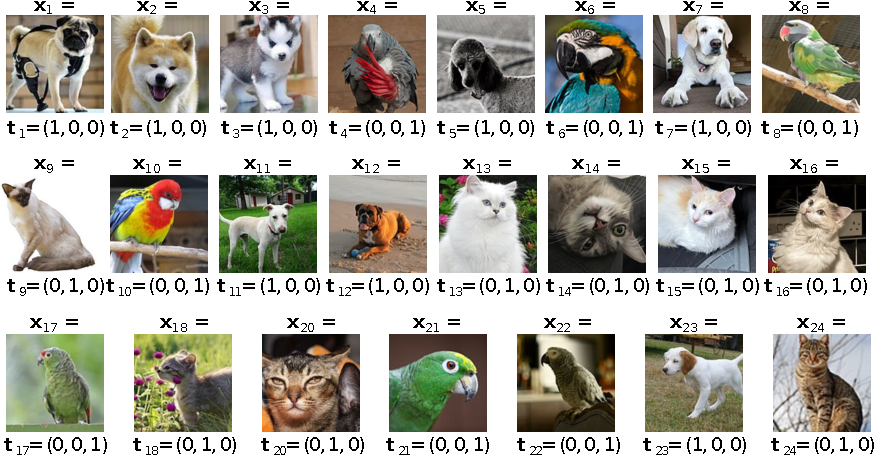
\includegraphics{media/learning_example_supervised.pdf}
	\caption{A supervised learning task. Given a set of $N$ examples mapping an image $\vec x_k$ onto a one-hot encoded category vector $\vec t_k$, we would like the computer to learn a mapping from unseen images $\vec x$ onto categories $\vec t$.}
	\label{fig:learning_example_supervised}
\end{figure}


Inspired by the learning abilities of biological systems, computer scientists have been working on \enquote{learning machines} since the early 1960s, giving rise to the field of machine learning. The main goal of this field is to apply computers to problems that have a less well-defined relationship between input and output.

\Example{Consider the following \enquote{image recognition} problem. A system receives an image encoded as a high-dimensional vector $\vec x$ (where each vector component corresponds to the intensity of one colour channel of a pixel in the image), and has to decide whether the image contains a dog, a cat, or a parrot (cf.~\cref{fig:learning_example_supervised}). It would be quite hard to write such a program \enquote{by hand}. After all, what are the rules by which we would categorize a set of pixels into these categories? The goal of machine learning is to be able to \enquote{program by example}. Instead of specifying an algorithm, we just specify examples, and the computer \enquote{figures out} (learns) on its own how to solve the problem in general.}

\newpage

Within this field, computer scientists typically distinguish between three types of learning:
\begin{itemize}
	\item \textbf{Supervised Learning}\\
	Given $N$ training samples $(\vec x_k, \vec t_k)$, and a model function $f(\vec x; \vec w)$, find weights/parameters $\vec w$ such that $f(\vec x_k) \approx \vec t_k$. We hope that after training, $f(\vec x; \vec w)$ will also work for unseen~$\vec x$. In other words, we assume that there is an unknown ground truth function $f_\mathrm{GT}(\vec x) = \vec t$ that we would like to approximate by tuning the parameters of our model function $f(\vec x; \vec w)$.\\
	\emph{Examples:} Polynomial fitting, Perceptrons, generalised linear models (GLMs), Support Vector Machines (SVMs), Gaussian Processes, Multi-Layer Perceptrons (MLPs).
	\item \textbf{Unsupervised Learning}\\
	We are just given a set of $N$ samples $\vec x_k$ and would like to discover some inherent order within this dataset. Sometimes, we would like to map each $\vec x_k$ onto a lower-dimensional \enquote{latent} space $\vec \lambda$, where conceptually similar $\vec x$ are being assigned to similar $\vec \lambda$.\\
	\emph{Examples:} Clustering, autoencoders, dimensionality-reduction methods (PCA, tSNE, \textellipsis).
	\item \textbf{Semi-supervised (or Reinforcement) Learning}\\
	A system receives state information $\vec x(t)$ and a low-dimensional reward signal $r(t)$. Goal is to learn a policy $\pi(\vec x)$ that produces actions $\vec t(t)$ maximizing the time-cumulative reward.
\end{itemize}

Furthermore, there are additional constraints on the learning process place that are orthogonal to these concepts, such as \enquote{offline} (training happens while the system is not being used), \enquote{online} (the system learns on a stream of data), or \enquote{life-long} (the system is constantly learning whenever it is active) learning.

In the following sections, we have a closer look at these concepts. Maybe we can borrow some insights from Machine Learning and apply them to our spiking neural network models!

\section{Supervised Learning}

As summarized above, the goal of supervised learning is to find parameters $\vec w$ for a model function $f(\vec x; \vec w)$, such that the function closely maps a set of $N$ training data points~$\vec x_k$ onto a set of desired target points~$\vec t_k$. The quality of the match is defined according to some loss function $E(\vec w)$. For example, if we assume a quadratic loss function, a supervised machine learning problem could be phrased as
\begin{align}
	\vec w &= \arg \min_{\vec w} E(\vec w) = \arg \min_{\vec w} \frac{1}{N} \sum_{k = 1}^N \big\| f(\vec x_k ; \vec w) - \vec t_k \big\|^2 \,.
	\label{eqn:supervised_learning}
\end{align}
While equation \cref{eqn:supervised_learning} looks quite innocuous, this problem is generally difficult because of the function~$f$. There is no constraint whatsoever on what $f$ should look like, except for the very general notion of $f$ being a function mapping from a $d$-dimensional input space $\mathbb{X} \subseteq \mathbb{R}^d$ onto some $d'$-dimensional target space $\mathbb{R}^{d'}$. Commonly used examples of model functions $f$ include
\begin{itemize}
	\item Polynomial of degree $n$: $f(\vec x; \vec w) = \sum_{i = 0}^n w_i x^i$.
	\item Linear models: $f(\vec x; \vec w) = \sum_{i = 0}^n w_i \phi_i(x)$.
	\item Perceptron: $f(\vec x; \mat w) = \phi\big(\langle \vec w, \vec x \rangle \big)$.
	\item Multi-layer perceptrons/\enquote{deep} neural networks.
\end{itemize}

The overall goal of this endeavour is \emph{generalisation}. While our training tuples $(\vec x_k, \vec t_k)$ may only cover a small portion of the space $\mathbb{X}$ we are interested in, the general hope is that once we find the right parameters $\vec w$, our function $f(\vec x; \vec w)$ will also work for tuples $(\vec x_k, \vec t_k)$ we have seen before. Underpinning this hope is the assumption that there exists a systematic mapping between $f_{\mathrm{GT}}(\vec x; \vec w)$ that is unknown to the engineer building the system, and that $f$ will approximate this $f_{\mathrm{GT}}$ after training.

Unfortunately, in general, there are not guarantees that this will actually work. To the contrary, we can guarantee that an algorithm solving for $\vec w$ that generalises well within one particular application domain will not be able to generalise will in another application domain. This is known as the so-called \enquote{No Free Lunch Theorem}.

\Note{\emph{Solving for decoders is a supervised learning problem.}
The problem we solve when computing identity or function decoders fits exactly into this framework. In this case, our function $f(\vec x; \vec w)$ is just a linear model given as
\begin{align*}
	f(\vec x; \vec w) &= \langle \vec w, \vec a(\vec x) \rangle \,,
\end{align*}
where $\vec w$ are our decoders, and $\vec a(\vec x)$ is the function mapping from an input $\vec x$ onto the neural activities. As we saw, we can just solve for the optimal $\vec w$ using the $L_2$-regularised Moore-Penrose pseudo inverse.}

\subsection{Using Gradient Descent to Solve for $\vec w$}

\begin{figure}
	\centering
	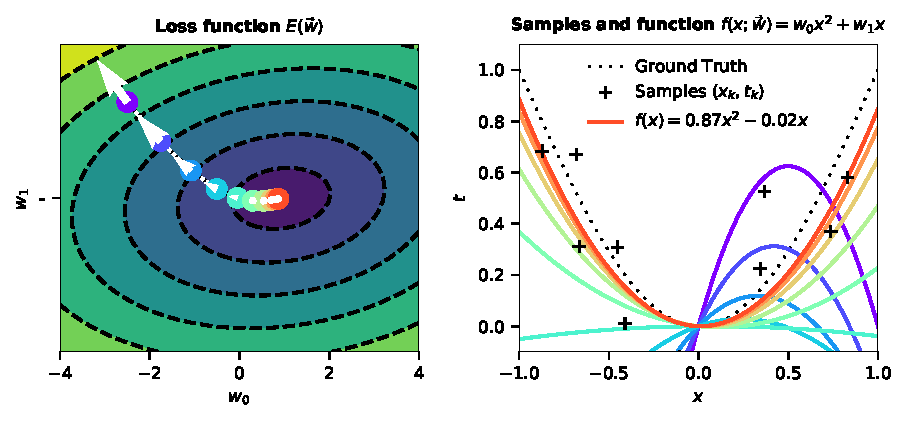
\includegraphics{media/gradient_descent_poly_example_10.pdf}
	\caption{Gradient descent in action. We are trying to find parameters for the polynomial model function $f(x; \vec w) = w_0 x^2 + w_1 x$ given a set of samples $(x_k, t_k)$. \emph{Left:} Loss function over the parameters $\vec w$, as well as the trajectory of the paramters $\vec w$ as part of the gradient descent algorithm. Arrows indicate the gradient $\Delta \vec w$. Brighter colours correspond to larger errors. \emph{Right:} Training samples $(x_k, t_k)$, as well as the parametrised model functions corresponding to the parameters highlighted in the left picture. \CodeLink{lecture_08/media/code/gradient_descent_example.ipynb}}
	\label{fig:gradient_descent_poly_example_10}
\end{figure}

In general, it is impossible to solve for $\vec w$ in closed form. Instead, computer scientists often fall back onto a heuristic known as \enquote{gradient descent}.

In a nutshell, we analyse how infinitesimally small changes to one of the weights $w_i$ would affect our loss function $E(\vec w)$. We use this information in order to apply a small change $- \eta \Delta \vec w$ to our weights, such that the error is being reduced. In particular, this change is given as
\begin{align*}
	\Delta w_i &= \big( \nabla E(\vec w) \big)_i =  \frac{\partial E(\vec w)}{\partial w_i} = \frac{\partial}{\partial w_i} \frac{1}{N} \sum_{k = 1}^N \big\| f(\vec x_k ; \vec w) - \vec t_k \big\|^2 \,, & \text{weight update step } \vec w &\gets \vec w - \eta \Delta \vec w \,,
\end{align*}
where $\eta$ is the so called \emph{learning rate}. The weight update steps are then repeated until $\vec w$ converges (i.e.,~does not change considerably). See \cref{fig:gradient_descent_poly_example_10} for a simple example, yet keep in mind that depending on $f(\vec x; \vec w)$ -- the loss function will not have a clear global minimum and the number of parameters can go into the thousands (and not just two as in the example).

We can either compute the partial differential $\frac{\partial}{\partial w_i}$ numerically (i.e., by evaluating $E$ for slightly different $\vec w$ and computing the difference quotient). For some $f$, the gradient $\nabla E$ can be evaluated efficiently using the chain-rule, leading to an algorithm called \emph{error back-propagation}. There are libraries such as Autograd or Tensorflow that conveniently compute these gradients.

In practice, the loss function $E$ is often not evaluated for all $N$ training samples at once, but for a random subset of $N' \ll N$ samples, where $N'$ is the so called \enquote{batch size}. Not only does this increase the efficiency of the gradient descent algorithm, it also prevents the algorithm from \enquote{getting stuck} in local minima. This variant of gradient descent is called \enquote{stochastic gradient descent} (stochastic because of the random selection of samples).

\subsection{The Delta Learning Rule}

As noted above, we are solving a supervised \enquote{learning} problem (in the machine learning sense) when computing decoders $\mat D$. However, so far we have been using what is known as an \emph{offline} method -- we compute $\mat D$ in one step for all $N$ using the $L_2$-regularised Moore-Penrose pseudo inverse. That is, we have a training phase during which we compute $\mat D$, followed by the \enquote{inference} phase during which we use $\mat D$ within our neural network.

In order to \emph{learn} synaptic weights $\mat W$ in the sense defined in the introduction, we need a so called \emph{online} learning rule. That is, we would like to find a learning rule that allows us to update the weights for a stream of input data while the network is active.

Luckily, we can easily derive such an algorithm in two stages. First, we will implement a decoder learning rule by performing gradient descent for an input-target pair $(\vec x(t), \vec y^\mathrm{d}(t))$. This is somewhat comparable to stochastic gradient descent with a batch size of $N' = 1$, although we do not randomly sample from a pool of $N$ available samples, but always use the information that is currently (i.e., at time $t$) available in our network.

Second, we will extend this \emph{decoder} learning rule to a biologically plausible \emph{synaptic weight} learning rule that updates individual entries of the weight matrix $w_{ij}$.

For simplicity, let's assume that $d = 1$, i.e., we are representing a scalar value. Now, our setup is as follows. We have a neuron population representing the input value $x$ and would like to decode an unknown function $f(x)$. In other words, we would like to continuously update our decoders $\vec d$, such that $f(x(t)) \approx y^\mathrm{d}(t)$. This means that we have the following loss function
\begin{align*}
	E(\vec d) &= \frac{1}2 \left(\left(\sum_{i = 1}^n d_i a_i\big(x(t)\big) \right) - y^\mathrm{d}(t) \right)^2 \\
	\Rightarrow \Delta d_i = \frac{\partial E(\vec d)}{\partial d_i} &= \underbrace{\left(\left(\sum_{i = 1}^n d_i a_i\big(x(t)\big) \right) - y^\mathrm{d}(t)\right)}_{\epsilon(t)} a_i\big(x(t)\big) \\
		&= \epsilon(t) a_i\big(x(t)\big) \,,
\end{align*}
where $\epsilon(t)$ is the error we are making at the current point in time. This is a version of the so called \enquote{Delta Learning Rule} for a linear model. In the next subsection we will extend this rule to individual synaptic weights $w_{ij}$.

\Note{Since we are not stochastically sampling from a large pool of $N$ samples, this method has a problem often referred to a \emph{catastrophic forgetting}. By not looking at older samples, we are temporarily over-fitting our system to the current region of the input-target space.}

\Aside{Stochastically sampling $(\vec x(t'), \vec y^\mathrm{d}(t'))$ pairs over a longer history $t' \in [t - \theta, t]$ using the Delay Network with the goal to increase the convergence rate and to somewhat mitigate the problem of catastrophic forgetting would be an interesting course project!}

\subsection{The Prescribed Error Sensitivity (PES) Learning Rule}

\begin{figure}
	\centering%
	\begin{subfigure}{0.5\textwidth}%
		\centering%
		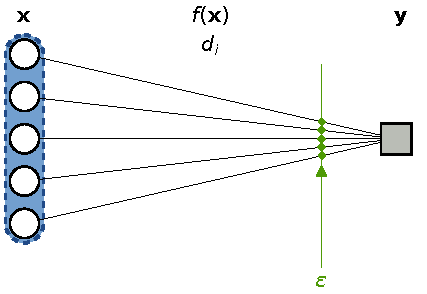
\includegraphics{media/pes_network_a.pdf}%
		\caption{Learning decoders}%
	\end{subfigure}%
	\begin{subfigure}{0.5\textwidth}%
		\centering%
		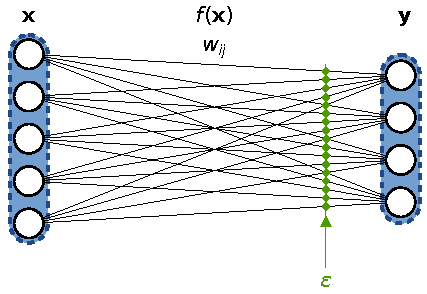
\includegraphics{media/pes_network_b.pdf}%
		\caption{Delta learning rule}%
	\end{subfigure}%
	\caption{Learning decoders $d_i$ \textbf{(a)} and synaptic weights \textbf{(b)} in an NEF network. We would like to learn an unknown function $\vec y = f(\vec x)$ encoded in either the decoding weights $d_i$ or in the weights between two neural populations. Weights are updated according to an error signal $\epsilon(t) = \vec y^\mathrm{d}(t) - y(t)$.}
\end{figure}

We now have a simple learning rule that allows us to learn decoders online -- essentially, we just multiply the neural activity $a_i(x(t))$ with the error $\epsilon(t)$ and then update individual decoder values according to the gradient descent update equation
\begin{align*}
	d_i \gets -\eta \Delta d_i = -\eta \epsilon(t) a_i(t) \,.
\end{align*}
Essentially, if a neuron is active while there is some positive error $\epsilon(t)$, we decrease its influence on the decoding. If there is a negative error $\epsilon(t)$, we increase its influence.

The problem with this equation is that it is not biologically plausible. There are no decoders in the brain, so we need to find a way to update synaptic weights $w_{ij}$ instead of decoders $d_i$.

However, this problem can be easily fixed. Remember that the synaptic weights are given as
\begin{align*}
	w_{ij} &= \big((\vec \alpha \circ \mat E) \mat D\big)_{ij} = \alpha_j \langle \vec e_j, \vec d_i \rangle \,.
\end{align*}
Substituting the decoder update $\Delta d_i$ into this equation (for the scalar case) gives us
\begin{align*}
	\Delta w_{ij} &= \alpha_j e_j \Delta d_i = - \eta \big( \alpha_j \epsilon(t) e_j \big) a_i(t) \,.
\end{align*}
For vectorial quantities $\vec x$ (i.e., $d > 1$) this just turns out to be
\begin{ImportantEqn}{Prescribed Error Sensitivity (PES) Learning Rule}
\Delta w_{ij} &= \alpha_j e_j \Delta d_i = -\eta \big( \alpha_j \langle \vec \epsilon(t), \vec e_j \rangle \big) a_i(t) \,.
\end{ImportantEqn}
Note that the term $\big( \alpha_j \langle \vec \epsilon(t), \vec e_j \rangle \big)$ looks very much like the linear part of the current-translation function in the NEF encoding equation. In particular, we are treating the error $\epsilon(t)$ as if it was an input $\vec x(t)$ -- and in a sense it is exactly that -- a so called \enquote{modulatory} input.

As it turns out, such modulatory inputs exist in the brain in the form of dopaminergic synapses, which enable synaptic plasticity in the post-synapse.

\subsection{Example: Supervised Learning of Functions $f$}

\begin{figure}[p]
	\centering
	\begin{subfigure}{\textwidth}
		\centering
		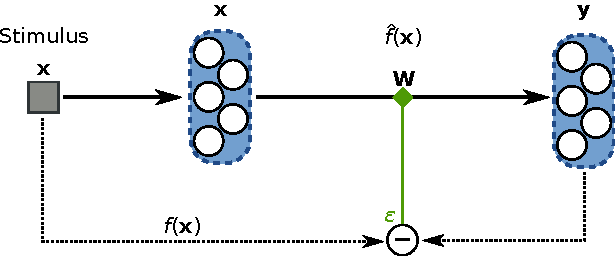
\includegraphics{media/learning_network.pdf}
		\caption{Network used for the learning experiments depicted below}
	\end{subfigure}
	\begin{subfigure}{\textwidth}
		\centering
		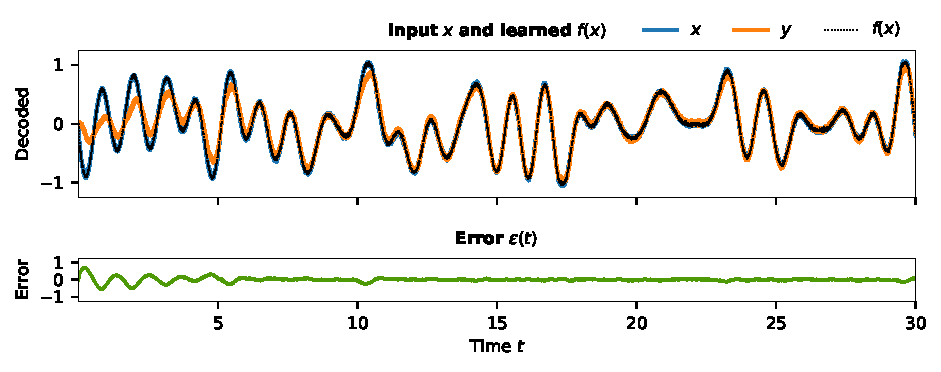
\includegraphics{media/pes_communication_channel_example.pdf}
		\caption{Learning $f(x) = x$}
		\label{fig:pes_communication_channel_example}
	\end{subfigure}
	\begin{subfigure}{\textwidth}
		\centering
		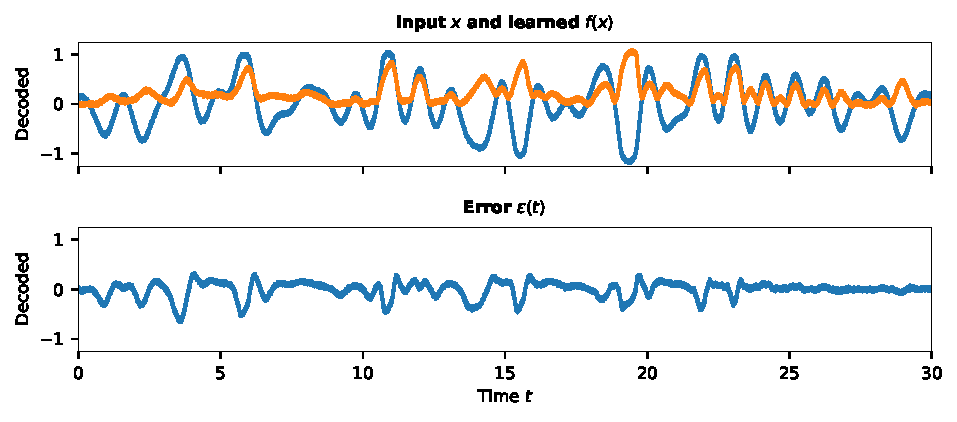
\includegraphics{media/pes_square_example.pdf}
		\caption{Learning $f(x) = x^2$}
		\label{fig:pes_square_example}
	\end{subfigure}
	\caption{\textbf{(a)} Network used for the learning experiment below. Blue boxes correspond to spiking neuron populations of $100$ neurons each. The learning rate is $\eta = 5 \times 10^{-5}$. \textbf{(b, c)} Learning different functions $f$ using the PES learning rule. Blue lines correspond to the decoding from the first neuron population representing $x$, orange lines correspond to the decoding from the second neuron population representing $y = \hat f(x)$. The black line corresponds to the optimal target $f(x)$. \CodeLink{lecture_08/media/code/pes_learning_rule_example.ipynb}}
	\label{fig:pes_learning_network}
\end{figure}

\Cref{fig:pes_learning_network} shows an example of learning a function $f(x) : \mathbb{R} \longrightarrow \mathbb{R}$, with an \enquote{artificially} created error signal $\epsilon(t)$. As clearly visible in \cref{fig:pes_communication_channel_example}, we are able to quickly learn a communication channel, i.e., $f(x) = x$, between two neuron populations.

Learning a more complex function such as $f(x) = x^2$ works as well, as depicted in \cref{fig:pes_square_example}. However, notice that learning progresses much slower in the second case. Correspondingly, we should note that not only the learning rate $\eta$ plays a role in how fast a function is being learned, but also the \enquote{complexity} of the function that is being learned.

\Note{We will have a closer look at why some functions may be harder to learn than others in the next lecture, when we analyse representations.}

\subsection{Example: Classical Conditioning}

\begin{figure}[t]
	\centering%
	\begin{subfigure}{0.5\textwidth}%
		\centering%
		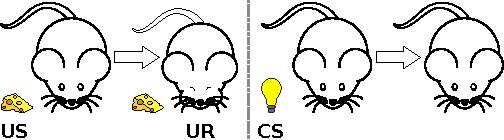
\includegraphics[scale=0.85]{media/classical_conditioning_a.pdf}%
		\caption{Before conditioning}%
	\end{subfigure}%
	\begin{subfigure}{0.5\textwidth}%
		\centering%
		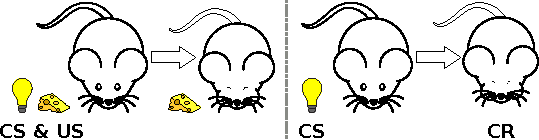
\includegraphics[scale=0.85]{media/classical_conditioning_b.pdf}%
		\caption{After conditioning}%
	\end{subfigure}\\[0.5cm]
	\begin{subfigure}{\textwidth}%
		\centering%
		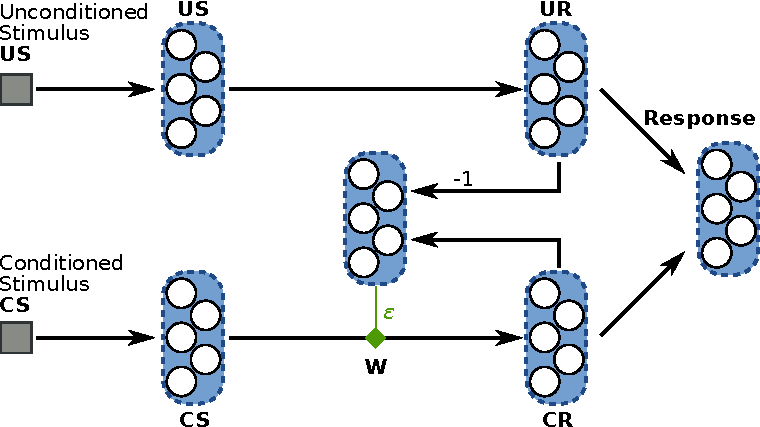
\includegraphics[scale=0.85]{media/conditioning_network.pdf}%
		\caption{Network model}
	\end{subfigure}\\[0.5cm]
	\begin{subfigure}{\textwidth}
		\centering
		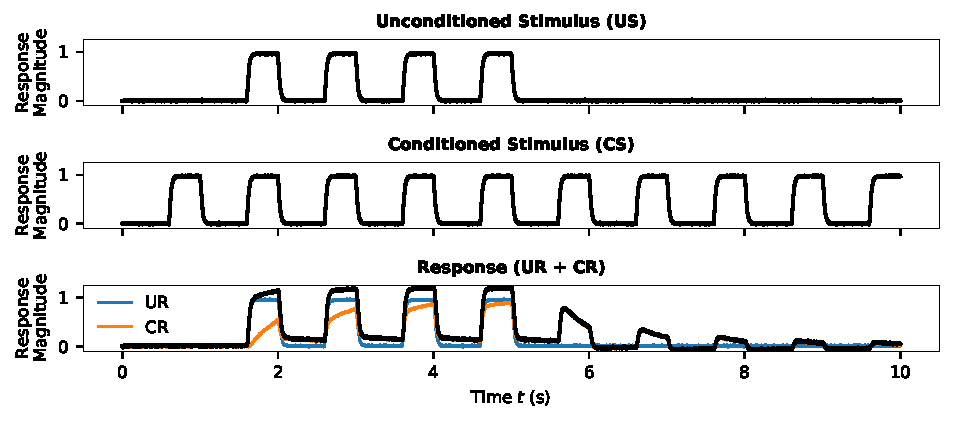
\includegraphics{media/classical_conditioning_experiment.pdf}
		\caption{Neural network implementing classical conditioning}
	\end{subfigure}
	\caption{Classical conditioning experiment. \textbf{(a, b)} Illustration of classical conditioning. An unconditioned stimulus (US, smell of cheese) causes an unconditioned response (UR, mouse is salviating). Paring a neutral conditioned stimulus (CS, light) with the unconditioned stimulus causes the animal to produce a conditioned response (CR). Adapted from \href{https://commons.wikimedia.org/wiki/File:Classical_conditioning_-_extinction.svg}{Wikimedia}. \textbf{(c)} Network model using the PES learning rule to implement classical conditioning.  \textbf{(d)} Graphs showing the values represented by the individual populations.}
\end{figure}

Classical conditioning is a phenomenon observed in human- and non-human animals, colloquially known through research performed by Ivan Pavlov on dogs (\enquote{Pavlov's dog}).

The general experimental setup is the following. An animal \enquote{unconditonally} (i.e.,~without initial training) responds to a stimulus. A well-studied example is the eye-blink reflex: here, an animal blinks whenever a \enquote{puff} of air is directed at their cornea. This stimulus-response pair is called \enquote{unconditioned stimulus} (US) and \enquote{unconditioned response} (UR).

If the unconditioned stimulus is paired with a so called conditioned stimulus (CS) (for example a tone, or a flash of light), the animal gradually learns to associate the conditioned stimulus with the unconditioned stimulus and will produce a conditioned response (CR) mimicking the unconditioned response even in the absence of the unconditioned stimulus.

One possible implementation of classical conditioning using the PES learning rule is given 

\subsection{Example: Adaptive Control}

\ConstructionSite

\section{Unsupervised Learning}

\ConstructionSite

\subsection{Principal Component Analysis}

\begin{itemize}
	\item \textbf{Basis Transformation} An orthonormal matrix $\mat T \in \mathbb{R}^{d \times d'}$ (\emph{orthonormal:} $\mat T \mat T^\T = \mat I$) is a so called \enquote{basis transformation}:
	\begin{itemize}
		\item $\vec \lambda = \mat T \vec x$
		\item $\vec x = \mat T^\T \vec \lambda$
	\end{itemize}
	$\vec \lambda$ and $\vec x$ contain exactly the same information, but from a different perspective.
	\item \textbf{Idea:} Find the $\mat T$ that packs the \enquote{most information} into the first dimensions.
	\item \textbf{Then:}
	\begin{itemize}
		\item \textbf{Can compress data}\\
			Can \enquote{throw away} (set to zero) coefficients $\lambda_i$ with $i > d'$
		\item \textbf{Can interpret the first dimensions}
	\end{itemize}
	\item This is exactly what Principal Component Analysis (PCA) does!
	\item PCA: Eigenvectors of the data covariance matrix sorted by the magnitude of the eigenvalue
	\item Algorithm:
	\begin{lstlisting}[language=python]
		# Input X: (N x d) array
		# Output T: (d x d) array
		X_cen = X - np.mean(X, axis=0)
		X_cov = (X_cen.T @ X_cen) / (N - 1)
		E, T = np.linalg.eigh(X_cov)
		# T sorted by magnitude of E
		T = T.T[::-1, :]
	\end{lstlisting}
\end{itemize}

\subsection{Unsupervised Hebbian Encoder Learning}

\begin{itemize}
	\item Hebbian Learning: \enquote{What fires together wires together}
	\item $\Delta w_{ij} = \eta a_i a_j$
	\item Problem: Unstable weights go to infinity
	\item BCM rule (Bienenstock, Cooper, \& Munro, 1982):
	\begin{align*}
		\Delta_{ij} = \eta a_i a_j (a_j - \theta)
	\end{align*}
	\item $\theta$: Activity Threshold (recent average activity of the pre-neuron)
	\item One can show: weights trained by the Hebbian Learning Rules converge to the first principal component
	\item \enquote{Encoder Learning}
	\item Active field of research; how to learn multiple PCA-like encoders in a biologically plausible manner?
\end{itemize}

\printbibliography

\end{document}

